\section*{Exercise 7.1}
The estimator of p is
\spl{
    \hat{p}=\frac{E}{n}=\frac{\overline{X}}{n}=\frac{0\cdot39+1\cdot23+2\cdot12+3\cdot1}{75\cdot24}=\frac{1}{36}.
}

The expected frequency can be calculated by $E_i=nP[X=i]=n\binom{n}{i}\hat{p}^i(1-\hat{p})^{n-i}$.
\begin{table}[H]
    \centering
    \begin{tabular}{ccccc}\hline
        Values & 0 & 1 & 2 & 3\\\hline
        Expected Frequency & 38.145 & 26.156 & 8.594 & 2.105\\\hline
    \end{tabular}
\end{table}

We notice that $E_i\geq5$ less than 80\% categories. Thus we merge the last two categories.
\begin{table}[H]
    \centering
    \begin{tabular}{ccccc}\hline
        Values & 0 & 1 & 2\\\hline
        Expected Frequency & 38.145 & 26.156 & 10.699\\\hline
    \end{tabular}
\end{table}

Then,we calculate the Pearson's Statistic
\spl{
    X^2=\sum_{i=1}^N\frac{(O_i-E_i)^2}{E_i}=\frac{(39-38.145)^2}{38.145}+\frac{(23-26.156)^2}{26.156}+\frac{(13-10.699)^2}{10.699}=0.876.
}

The degree of freedom is $3-1-1=1$. Hence, $X^2=0.876<\chi^2_{0.05,1}=3.84$. Hence, we conclude that follows binomial distribution at 5\% level of significance.

\section*{Exercise 7.2}
\begin{table}[h]
    \centering
    \begin{tabular}{c|cccc|c}
        Mounting Position & A & B & C & D & \\\hline
        1 & 22 & 46 & 18 & 9 & 95\\
        2 & 4 & 17 & 6 & 12 & 39\\\hline
        & 26 & 63 & 24 & 21 & 134\\
    \end{tabular}
\end{table}

\spl{
    H_0:\ p_{ij}=p_{i\cdot}p_{\cdot j}
}

Since $E_{ij}=\frac{n_{i\cdot}n_{\cdot j}}{n}$, then
\spl{
    E_{11}&=18.43,\quad E_{12}=44.66,\quad E_{13}=17.01,\quad E_{14}=14.88\\
    E_{21}&=7.57,\quad E_{22}=18.34,\quad E_{23}=6.99,\quad E_{24}=6.11\\
}

\spl{
    X_{(2-1)(4-1)}^2=\sum_{i=1}^r\sum_{j=1}^c\frac{(O_{ij}-E_{ij})^2}{E_{ij}}=10.71.
}

Since the statistic follows 3 degrees of freedom chi-squared distribution, we compare the value with $\chi_{0.05,3}^2=7.8147$. We find that $X_3^2>\chi_{0.05,3}^2$. Thus, we reject the hypothesis at 5\% level of significance. We claim that the type of failure depends on the mounting position.

\section*{Exercise 7.3}
\begin{table}[h]
    \centering
    \begin{tabular}{c|ccccc|c}
        & 1 & 2 & 3 & 4 & 5 &\\\hline
        Male & 50 &47 & 103 & 76 & 24 & 300\\
        Female & 21 & 27 & 50 & 35 & 17 & 150\\\hline
        & 71 & 74 & 153 & 111 & 41 & 450\\
    \end{tabular}
\end{table}
We assume that the increase in the salary is independent od the workers' gender, saying that
\spl{
    H_0:\ p_{ij}=p_{i\cdot}p_{\cdot j}
}

Since $E_{ij}=\frac{n_{i\cdot}n_{\cdot j}}{n}$, then
\spl{
    E_{11}&=47.33,\quad E_{12}=49.33,\quad E_{13}=102,\quad E_{14}=74,\quad E_{15}=27.33\\
    E_{21}&=23.67,\quad E_{22}=24.67,\quad E_{23}=51,\quad E_{24}=37,\quad E_{25}=13.67\\
}

\spl{
    X_{(2-1)(5-1)}^2=\sum_{i=1}^r\sum_{j=1}^c\frac{(O_{ij}-E_{ij})^2}{E_{ij}}=2.19.
}

Since the statistic follows 4 degrees of freedom chi-squared distribution, we compare the value with $\chi_{0.05,4}^2=9.4877$. We find that $X_4^2<\chi_{0.05,3}^2$. Thus, we support the hypothesis at 5\% level of significance. We claim that increase in salary is independent of the gender.

\section*{Exercise 7.4}
Using the Helmert transformation $\textbf{Y}\rightarrow\textbf{D}$, we rewrite $SSE_{pe}$
\spl{
    SSE_{pe}&=\frac{1}{\sigma^2}\sum_{i=1}^k\sum_{j=1}^{n_i}(Y_{ij}-\overline{Y_{ij}})^2\\
    &=\frac{1}{\sigma^2}\sum_{i=1}^k\bigg[\sum_{j=1}^{n_i}Y_{ij}^2-n_i\overline{Y_{ij}}^2\bigg]\\
    &=\frac{1}{\sigma^2}\sum_{i=1}^k\bigg[\sum_{j=1}^{n_i}D_{ij}^2-D_{i1}^2\bigg]\\
    &=\frac{1}{\sigma^2}\sum_{i=1}^k\bigg[\sum_{j=2}^{n_i}D_{ij}^2\bigg]\\
    &=\frac{1}{\sigma^2}\bigg[\sum_{i=1}^nD_i^2-\sum_{i=1}^kD_{i1}^2\bigg]\\
    &=\sum_{i=1}^n\frac{D_i^2}{\sigma^2}-\sum_{i=1}^k\frac{D_{i1}^2}{\sigma^2},
}
which is the sum of square of $(n-k)$ normally distributed variables. Hence, it follows $(n-k)$ degrees of freedom chi-squared distribution.

\section*{Exercise 7.5}
Consider $\cov(\overline{Y},\hat{\beta}_1)$, we obtain
\spl{
    \hat{\beta}_1&=B_1=\frac{S_{xy}}{S_{xx}}\\
    \cov(\overline{Y},\hat{\beta}_1)&=E[\overline{Y}\hat{\beta}_1]-E[\overline{Y}]E[B_1]\\
    &=E\bigg[\frac{\sum_{i=1}^n(x_i-\bar{x})Y_i\overline{Y}}{\sum_{i=1}^n(x_i-\bar{x})^2}\bigg]-(\beta_0+\beta_1\bar{x})\beta_1\\
    &=\frac{\sum_{i=1}^n(x_i-\bar{x})E[Y_i\overline{Y}]}{\sum_{i=1}^n(x_i-\bar{x})^2}-(\beta_0+\beta_1\bar{x})\beta_1\\
    &=\frac{\sum_{i=1}^n(x_i-\bar{x})(\beta_0+\beta_1 x_i)(\beta_0+\beta_1\bar{x})}{\sum_{i=1}^n(x_i-\bar{x})^2}-(\beta_0+\beta_1\bar{x})\beta_1\\
    &=0
}

Consider $\cov(\hat{\beta_0},\hat{\beta_1})$, we obtain
\spl{
    \cov(\hat{\beta_0},\hat{\beta_1})&=E[B_0B_1]-E[B_0]E[B_1]\\
    &=E[(\overline{Y}-B_1\bar{x})B_1]-\beta_0\beta_1\\
    &=E[B_1\overline{Y}-B_1^2\bar{x}]-\beta_0\beta_1\\
    &=E[B_1\overline{Y}]-E[B_1^2\bar{x}]-\beta_0\beta_1\\
    &=(\beta_0+\beta_1\bar{x})\beta_1-\bar{x}E[B_1^2]-\beta_0\beta_1\\
    &=\bar{x}(\beta_1^2-E[B_1^2])\\
    &=-\bar{x}(E\bigg[(\frac{S_{xy}}{S_{xx}})^2\bigg]-E\bigg[\frac{S_{xy}}{S_{xx}}\bigg]^2)\\
    &=-\bar{x}\var(B_1)\\
    &=-\bar{x}\frac{\sigma^2}{S_{xx}}\\
    &=-\frac{\bar{x}}{S_{xx}}\sigma^2.
}

\section*{Exercise 7.6}
\enum{
\item
\spl{
    B_1&=\frac{S_{xy}}{S_{xx}}=184.6\\
    B_0&=\overline{Y}-B_1\bar{x}=-2150
}
\item
\spl{
    S^2=\hat{\sigma}^2=\frac{S_{yy}-B_1S_{xy}}{n-2}=1.15\e{5}.
}
\item
For a 100(1-0.1)\% confidence interval,
\spl{
    B_1\pm t_{0.1/2,n-2}\frac{S}{\sqrt{S_{xx}}}&=184.6\pm1.68\cdot\frac{339.2185}{\sqrt{828.2412}}=184.6\pm19.8.\\
    B_0\pm t_{0.1/2,n-2}\frac{S\sqrt{\sum x_i^2}}{\sqrt{nS_{xx}}}&=-2150\pm1.68\cdot\frac{339.2185\cdot182.8296}{\sqrt{42\cdot828.2412}}=-2150\pm560.\\
}
\item
\spl{
    &H_0:\ \text{the linear regression is appropriate}\\
    &H_1:\ \text{the linear regression is not appropriate}
}
\spl{
    SSE_{pe}&=\sum_{i=1}^k\sum_{j=1}^{n_i}(Y_{ij}-\overline{Y}_i)^2=109500.\\
    SSE_{lf}&=SSE-SSE_{pe}=4.49\e{6}.
}
Hence,
\spl{
    F_{37-2,42-37}=\frac{4.49\e{6}/(37-2)}{109500/(42-37)}=5.8621
}

Since $f_{0.05,35,5}=4.4775<F_{35,5}$, then we claim that the linear regression model is not appropriate at 5\% level of significance.

\item
\spl{
    R^2=\frac{S_{yy}-SSE}{S_{yy}}=0.8597.
}
The coefficient of determination is the proportion in $S_{yy}$ that is determined by $X$. The larger $R^2$ is, the more $Y$ are determined by $X$.

\item
\begin{figure}[H]
    \centering
    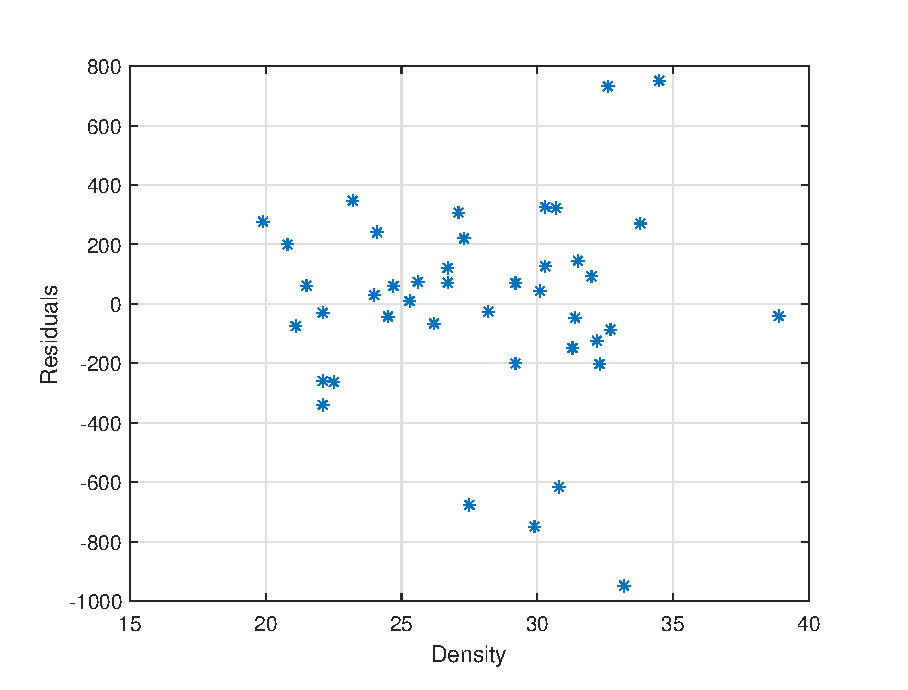
\includegraphics[height=9cm]{images/1}
    \caption{Residuals vs. Density}
\end{figure}
The assumption of constant variance is unreliable because the is irregular.
}

\section*{Exercise 7.7}
\enum{
\item
\begin{figure}[H]
    \centering
    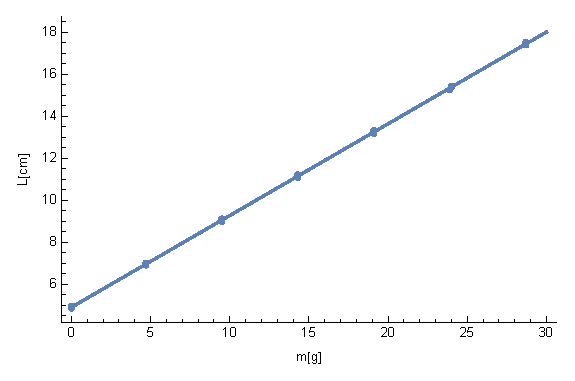
\includegraphics[height=9cm]{images/2}
    \caption{Linear regression model}
\end{figure}

\item
\spl{
    R^2=\frac{S_{yy}-SSE}{S_{yy}}=0.9998.
}
Hence,
\spl{
    \frac{R\sqrt{n-2}}{\sqrt{1-R^2}}=191.994>t_{0.025,12}=2.18.
}
It implies that our linear regression model is appropriate.

\item
\spl{
    &H_0:\ \text{the linear regression is appropriate}\\
    &H_1:\ \text{the linear regression is not appropriate}
}
\spl{
    SSE_{pe}&=\sum_{i=1}^k\sum_{j=1}^{n_i}(L_{ij}-\overline{L}_i)^2=0.0322.\\
    SSE_{lf}&=SSE-SSE_{pe}=0.0398547-0.0322=0.00765.
}
Hence,
\spl{
    F_{8-2,14-8}=\frac{0.00765/(8-2)}{0.0322/(14-8)}=0.2376.
}

Since $f_{0.05,6,6}=4.2839>F_{6,6}$, then we claim that the linear regression model is appropriate at 5\% level of significance.
}

\section*{Exercise 7.8}
\spl{
    \textbf{LHS}-\textbf{RHS}&=\frac{S_{xy}}{S\sqrt{S_{xx}}}-\frac{\sqrt{n-2}S_{xy}/\sqrt{S_{xx}S_{yy}}}{\sqrt{1-S_{xy}^2/S_{xx}S_{yy}}}\\
    &=\frac{S_{xy}}{S\sqrt{S_{xx}}}-\frac{\sqrt{n-2}S_{xy}}{\sqrt{S_{xx}S_{yy}-S_{xy}^2}}\\
    &=\frac{S_{xy}}{\sqrt{(S_{xx}S_{yy}-S_{xy}^2)/(n-2)}}-\frac{\sqrt{n-2}S_{xy}}{\sqrt{S_{xx}S_{yy}-S_{xy}^2}}\\
    &=\frac{\sqrt{n-2}S_{xy}}{\sqrt{S_{xx}S_{yy}-S_{xy}^2}}-\frac{\sqrt{n-2}S_{xy}}{\sqrt{S_{xx}S_{yy}-S_{xy}^2}}\\
    &=0.\\
}